%
% ee.tex
% Gunther Abbot
% 2019
%

\documentclass[letterpaper, 11pt]{report}

% Packages
\usepackage{amsmath,amssymb,amsfonts,amsthm}
\usepackage[hidelinks]{hyperref}
\usepackage{marginnote} % margin notes
\usepackage{fancyhdr} % fancy header
\usepackage{tocloft}
\usepackage{setspace}
\usepackage{graphicx}
\usepackage{amsmath}
\usepackage{mathtools} % Equation comments
\usepackage{soul}
\usepackage{paralist}
\usepackage{float}
\usepackage{todonotes}
%\usepackage{geometry}
\usepackage{xcolor}         % Extended colors
\usepackage{color}         % Color extended names
\usepackage[siunitx]{circuitikz}
\usepackage{apacite}
%\usepackage{tcolorbox}
%\tcbuselibrary{theorems}
%\tcbuselibrary{breakable}
%\tcbset{colback=white}

\definecolor{boxcolor}{HTML}{efefef}

\newcommand{\note}[1]{\intertext{#1}}
\newcommand{\hll}[1]{\colorbox{yellow}{$\displaystyle #1$}} % Equation highlighting

\pagestyle{fancy}
%\renewcommand{\sectionmark}[1]{\markright{#1}}
%\renewcommand*{\sectionmark}[1]{ \markright{\thesection\ ##1} }%
\renewcommand{\chaptermark}[1]{\markboth{#1}{}}
\renewcommand{\sectionmark}[1]{\markright{#1}{}}
\fancyhf{}
\rhead{\nouppercase{\rightmark}}
\lhead{\nouppercase{\leftmark}}
%\fancyhead[L]{}
%\fancyhead[R]{\rightmark}
\cfoot{\thepage}

\renewcommand*{\thefootnote}{(\arabic{footnote})}

%\newenvironment{mybox}[1]%
%{%
%	\addtocounter{subsection}{1}%
%	\addcontentsline{toc}{subsection}{\protect\numberline{\thesubsection}#1}%
%	\begin{tcolorbox}[title=#1]%
%	\abovedisplayskip=0pt%
%	\belowdisplayskip=0pt%
%}{%
%	\end{tcolorbox}%
%}%

%\newtcolorbox{equationframe}[1]{ams align*, title=#1}

%\newenvironment{name}[args]{begdef}{enddef}
%\newenvironment{myboxy}[1]%
%{%
%	\addtocounter{subsection}{1}%
%	\addcontentsline{toc}{subsection}{\protect\numberline{\thesubsection} #1}%
%	\begin{equationframe}{#1}%
%%	\abovedisplayskip=0pt%
%%	\belowdisplayskip=0pt%
%}{%
%	\end{equationframe}%
%}

\newcolumntype{L}{>{$}l<{$}} % math-mode version of "l" column type


% \newtheorem{<name>}{<heading>}[<counter>]
%\newtheorem{formula}{Formula}[section]
%\newtcbtheorem{theorem}{Theorem}{ams align*}{thm}

\setcounter{secnumdepth}{4}
\setcounter{tocdepth}{5}

%\renewcommand{\cftchapnumwidth}{6em}

%% Document
\begin{document}
	
%% Title Page
\pagenumbering{roman}
%\begin{titlepage}
%	\center\vspace*{3cm}
%	
%	\begin{spacing}{1.2}
%		\LARGE ECE 2630\\ ECE 2660%\\ ECE 3750
%	\end{spacing}
%	\vspace*{2em}
%	Gunther Abbot
%	
%	\vfill
%	{\small 2019\\ Last updated \today}
%\end{titlepage}
\begin{titlepage}
	\center\vspace*{1cm}
	
	\begin{center}
		\fbox{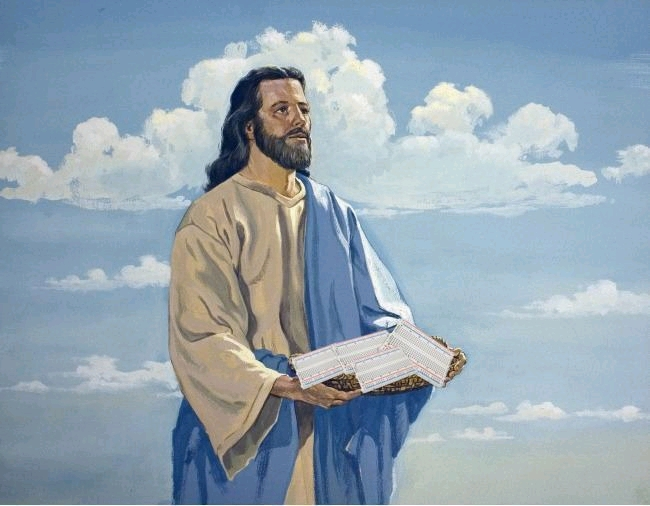
\includegraphics[width=0.8\textwidth]{ee.jpeg}}
	\end{center}
	\vspace*{2em}
	{\LARGE Electrical Engineering Notes}
	
	\vspace*{1em}
	Gunther Abbot
	
	\vfill
	{\small 2019\\ Last updated \today}
\end{titlepage}
\tableofcontents


\chapter*{Foreword}\addcontentsline{toc}{chapter}{Forword}

If I were to ask you what you think an electrical engineer is or does, you might answer “An electrical engineer is someone who solves problems that involve electricity.” But, if a friend replaces a light bulb, does that make my friend an electrical engineer? If you intuitively answer no, even if you can’t quite express why, that’s OK. One of my goals for you in this course is to help you to better understand what an electrical engineer is and does, and as a result be able to explain why my friend is not an electrical engineer (with which I agree, by the way).

One of the primary differences between engineers and people who solve problems \textit{ad hoc} (which by the way is everyone, in some sense) is that engineers tend to use a systematic, strategic approach to problem-solving, which includes the ability to test the problem solution to ensure that 1) you solve the correct problem, and 2) you solved the problem correctly. Another of my goals for you is to develop such a strategic, systematic approach to solve problems whose solutions involve processing information of an electrical nature.

But, a good solution to a problem is only as good as your ability to communicate it clearly, concisely, and effectively to others. Another goal of mine for you is to develop such communication skills, both in writing and in speaking, so that others will read and hear what you intend to communicate.

So, why bother with all of this?  After all, it sounds like a lot of really difficult work – and it is. But, my overarching goal for you in this course is for you to have the knowledge, skills, and the habit of careful, rigorous attention to detail that make you more attractive to potential employers at the end of the semester than at the beginning.  After all, light bulbs aren’t free!

\hfill \textemdash Todd DeLong

\pagenumbering{arabic}
%% Body
\part{Signals \& Systems}
%\chapter{Signals \& Systems}

\section{Fourier Series}

Cosine/Sine Representation
\begin{align*}
&f(t) = a_0 + \sum_{n=1}^{\infty}\left[a_n \cos(2\pi nf_0 t) + b_n \sin(2\pi nf_0 t)\right],\; f_0 = \frac{1}{T}\\
&a_0 = \frac{1}{T}\int_{0}^{T}f(t)dt, \qquad a_n = \frac{2}{T}\int_{0}^{T}f(t)\cos(2\pi nf_0 t)dt,\\
&b_n = \frac{2}{T}\int_{0}^{T} f(t)\sin(2\pi nf_0 t)dt\\
\end{align*}
Amplitude/Phase Representation
\begin{align*}
&f(t) = a_0 + \sum_{n=1}^{\infty}c_n \cos(2\pi nf_0 + \phi_n),\; f_0 = \frac{1}{T}\\
&a_0 = \frac{1}{T}\int_{0}^{T}f(t)dt, \quad c_n = \sqrt{a_n^2 + b_n^2}\\
&\phi_n = \begin{cases}
-\arctan(b_n / a_n) & a_n > 0\\
\pi -\arctan(b_n / a_n) & a_n < 0\\
\end{cases}
\end{align*}
Exponential Representation
\begin{gather*}
f(t)=\sum_{n=-\infty}^{\infty}\mathbf{x}_n e^{jn\omega_0 t}\\
\mathbf{x}_n=\left|\mathbf{x}_n\right|e^{j\phi_n}, \quad \mathbf{x}_{-n}=\mathbf{x}_n^*, \quad \phi_{-n}=-\phi_n, \quad \left|\mathbf{x}_n\right|=c_n/2, \quad x_0=c_0 \\
\mathbf{x}_n=\frac{1}{T_0}\int_{0}^{T_0}x(t)e^{-jn\omega_0 t}dt
\end{gather*}



%\begin{mybox}{Fourier Series}
%	Cosine/Sine Representation
%	\begin{align*}
%	&f(t) = a_0 + \sum_{n=1}^{\infty}\left[a_n \cos(2\pi nf_0 t) + b_n \sin(2\pi nf_0 t)\right],\; f_0 = \frac{1}{T}\\
%	&a_0 = \frac{1}{T}\int_{0}^{T}f(t)dt, \qquad a_n = \frac{2}{T}\int_{0}^{T}f(t)\cos(2\pi nf_0 t)dt,\\
%	&b_n = \frac{2}{T}\int_{0}^{T} f(t)\sin(2\pi nf_0 t)dt\\
%	\end{align*}
%	Amplitude/Phase Representation
%	\begin{align*}
%	&f(t) = a_0 + \sum_{n=1}^{\infty}c_n \cos(2\pi nf_0 + \phi_n),\; f_0 = \frac{1}{T}\\
%	&a_0 = \frac{1}{T}\int_{0}^{T}f(t)dt, \quad c_n = \sqrt{a_n^2 + b_n^2}\\
%	&\phi_n = \begin{cases}
%	-\arctan(b_n / a_n) & a_n > 0\\
%	\pi -\arctan(b_n / a_n) & a_n < 0\\
%	\end{cases}
%	\end{align*}
%\end{mybox}

\section{Fourier Transform}
\begin{align*}
F\left[x(t)\right] &= X(\omega) = \int_{-\infty}^{\infty}x(t)e^{-j\omega t}dt \\
x(t) &= F^{-1}\left[X(\omega)\right] = \frac{1}{2\pi}\int_{-\infty}^{\infty}X(\omega)e^{-j\omega t}d\omega
\end{align*}

\section{Convolution}
\[x(t) * h(t) = \int_{-\infty}^{\infty}x(\tau)h(t-\tau)d\tau\]

%\begin{mybox}{Fourier Transform}
%\begin{align*}
%F\left[x(t)\right] &= X(\omega) = \int_{-\infty}^{\infty}x(t)e^{-j\omega t}dt \\
%x(t) &= F^{-1}\left[X(\omega)\right] = \frac{1}{2\pi}\int_{-\infty}^{\infty}X(\omega)e^{-j\omega t}d\omega
%\end{align*}
%Hey there
%\end{mybox}

%\begin{mybox}{Convolution Integral}
%\[x(t) * h(t) = \int_{-\infty}^{\infty}x(\tau)h(t-\tau)d\tau\]
%Other stuff
%\end{mybox}

\chapter{Linear Time-Invariant Systems}


\section{Convolution}
\[x(t) * h(t) = \int_{-\infty}^{\infty}x(\tau)h(t-\tau)d\tau\]

\chapter{Frequency-Domain Analysis}
Summary of analysis techniques:
\begin{itemize}
	\item Phasor Analysis: Requires sinusoid, single frequency (per source), steady state
	\item Fourier Analysis: 
	\begin{itemize}
		\item Fourier Series: Requires periodic, steady state signals, but can handle non-sinusoidal signals
		\item Fourier Transform: Requires steady state (can handle non-periodic)
	\end{itemize}
	\item Laplace Analysis: Most general in that it allows for transient inputs
\end{itemize}


\section{Phasor Analysis}

\section{Fourier Series}

Cosine/Sine Representation
\begin{align*}
&f(t) = a_0 + \sum_{n=1}^{\infty}\left[a_n \cos(2\pi nf_0 t) + b_n \sin(2\pi nf_0 t)\right],\; f_0 = \frac{1}{T}\\
&a_0 = \frac{1}{T}\int_{0}^{T}f(t)dt, \qquad a_n = \frac{2}{T}\int_{0}^{T}f(t)\cos(2\pi nf_0 t)dt,\\
&b_n = \frac{2}{T}\int_{0}^{T} f(t)\sin(2\pi nf_0 t)dt\\
\end{align*}
Amplitude/Phase Representation
\begin{align*}
&f(t) = a_0 + \sum_{n=1}^{\infty}c_n \cos(2\pi nf_0 + \phi_n),\; f_0 = \frac{1}{T}\\
&a_0 = \frac{1}{T}\int_{0}^{T}f(t)dt, \quad c_n = \sqrt{a_n^2 + b_n^2}\\
&\phi_n = \begin{cases}
-\arctan(b_n / a_n) & a_n > 0\\
\pi -\arctan(b_n / a_n) & a_n < 0\\
\end{cases}
\end{align*}
Exponential Representation
\begin{gather*}
f(t)=\sum_{n=-\infty}^{\infty}\mathbf{x}_n e^{jn\omega_0 t}\\
\mathbf{x}_n=\left|\mathbf{x}_n\right|e^{j\phi_n}, \quad \mathbf{x}_{-n}=\mathbf{x}_n^*, \quad \phi_{-n}=-\phi_n, \quad \left|\mathbf{x}_n\right|=c_n/2, \quad x_0=c_0 \\
\mathbf{x}_n=\frac{1}{T_0}\int_{0}^{T_0}x(t)e^{-jn\omega_0 t}dt
\end{gather*}



\section{Fourier Transform}
\begin{align*}
F\left[x(t)\right] &= X(\omega) = \int_{-\infty}^{\infty}x(t)e^{-j\omega t}dt \\
x(t) &= F^{-1}\left[X(\omega)\right] = \frac{1}{2\pi}\int_{-\infty}^{\infty}X(\omega)e^{-j\omega t}d\omega
\end{align*}

\subsection{Unilateral Laplace Transform}

\[X(s)=\mathcal{L}\left[x(t)\right]=\int_{0^-}^{\infty}x(t)e^{-st}dt, \quad s=\sigma+j\omega\]
\chapter{Filters}

\section{Second-Order Low Pass}
Generalized equation:
\[H(s)=\frac{K}{1+\left(\frac{s}{\omega_0}\right)\frac{1}{Q} + \left(\frac{s}{\omega_0}\right)^2} = \frac{\omega_0^2}{s^2 + \frac{\omega_0}{Q}s + \omega_0^2}\]

\section{Quality Factor \& Damping}
Tells us the quality of our energy storage components and how close they are to their ideal versions.
\[Q=\frac{\text{Energy stored}}{\text{Energy lost per cycle}}\]
Energy storage equations for a capacitor and an inductor:
\[U_C=\frac{1}{2}CV^2 \quad U_L=\frac{1}{2}LI^2\]
\subsection{Derivation of Q factor for an RLC circuit}
Energy stored in the inductor:
\[U=\frac{1}{2}LI^2\]
Energy dissipated in the resistor:\footnote{I dont know where this equation comes from}
\[U=\frac{1}{2}I^2 R/\omega_0\]
So the quality factor is:
\[Q=\frac{\frac{1}{2}LI^2}{\frac{1}{2}I^2 R/\omega_0}=\frac{\omega_0 L}{R}\]
Since the resonant frequency is:
\[\omega_0=\frac{1}{\sqrt{LC}}\]
The Q factor for an RLC circuit is
\[Q=\frac{1}{R}\sqrt{\frac{L}{C}}\]

\subsection{Damping}
Damping is a time domain phenomenon, and refers to the step response.
\begin{align*}
Q<0.5:&\text{ Overdamped}\\
Q>0.5:&\text{ Underdamped}\\
Q=0.5:&\text{ Critically damped}\\
\end{align*}




\section{Butterworth Characteristic}
For a second-order low/high pass filter, this is the Q factor that makes the frequency response maximally flat. The value is:
\[Q=\frac{1}{\sqrt{2}}=\frac{\sqrt{2}}{2}=0.707\]

\section{Sallen-Key, Second-Order}
Equations:\footnote{$Q$ and $\omega_0$ are found by comparing the transfer function to standard form}
\begin{gather*}
H(s)=\frac{V_{out}}{V_{in}}=\frac{K}{s^2 R_1 R_2 C_1 C_2 + s\left[R_1 C_2 + R_2 C_2 + R_1 C_1\left(1-K\right)\right]+1}\\
\omega_0=\frac{1}{\sqrt{R_1 R_2 C_1 C_2}} \qquad Q = \frac{\sqrt{R_1 R_2 C_1 C_2}}{R_1 C_2 + R_2 C_2 + R_1 C_1\left(1-K\right)}
\end{gather*}
Designing a Sallen-Key filter:
\begin{enumerate}
	\item Determine the gain of the system, $K$. If unity-gain, $K=1$. Values of $R_A$ and $R_B$ can be determined here.
	\item Usually given a corner frequency and a Q factor, e.g. $\frac{\sqrt{2}}{2}=0.707$. Use the ratio method to find values of $m$ and $n$ that equal this Q factor:
	\[Q=\frac{\sqrt{mn}}{m+1}\]
	\item Choose values of $R$ and $C$ to match the desired corner frequency using these new values $m$ and $n$:
	\[\omega_0=\frac{1}{\sqrt{mn}RC}\]
	\item Then use the ratios to find the values of $R_1$ and $C_1$:
	\begin{align*}
	R_2 &= R & C_2 &= C\\
	R_1 &= mR & C_1 &= nC \\
	\end{align*}
\end{enumerate}













\part{Circuits \& Electronics}
\chapter{Operational Amplifiers}

\section{Basic Configuration}

\section{Non-inverting}
\begin{figure}[H]
	\centering
	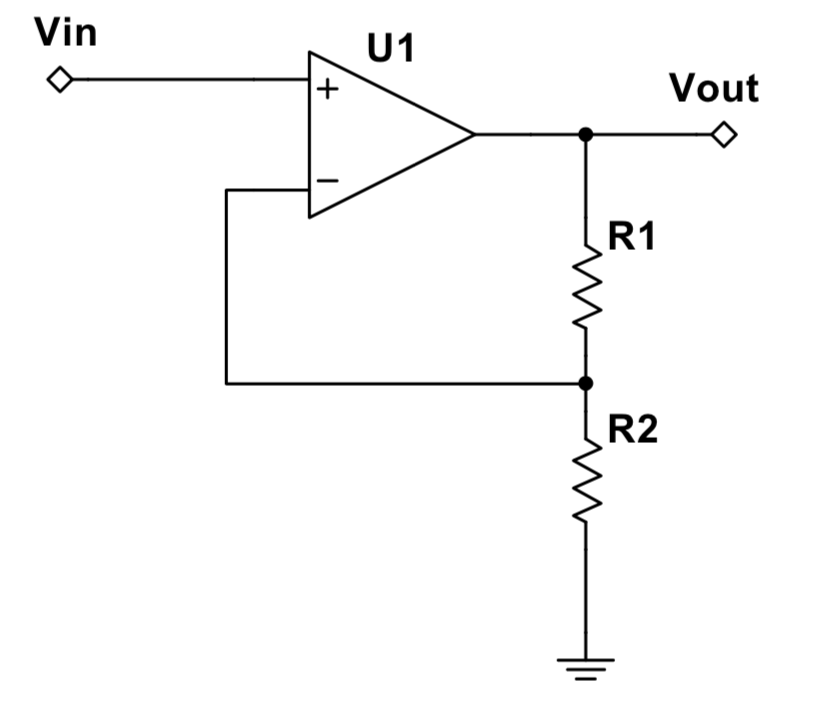
\includegraphics[width=2in]{opamps/noninverting.png}
%	\caption{Non-inverting}
	\label{fig:fig}
\end{figure}
Gain equation:
\[\frac{V_{out}}{V_{in}} = \frac{R_2 + R_1}{R_2} \]
%\begin{figure}
%	\begin{center}
%		\begin{circuitikz}
%			\draw (0,0) node[op amp] (opamp) {}
%			(opamp.-) to [R, l_=$R_1$, *-o] ($(opamp.-)-(2,0)$) node[left]{$V_{in}$}
%			(opamp.-) |- ($(opamp.-)+(0.2,1)$) to[R=$R_2$] ($(opamp.-)+(2.2,1)$) -|
%			(opamp.out) to[short,*-] ($(opamp.out)+(.5,0)$) node [right] {$V_{out}$} node [ocirc] {} 
%			(opamp.+) to[short]  ($(opamp.+)-(0,.5)$) node[ground] {}
%			;
%		\end{circuitikz}
%	\end{center}
%\end{figure}

\section{Inverting}
\begin{figure}[H]
	\centering
	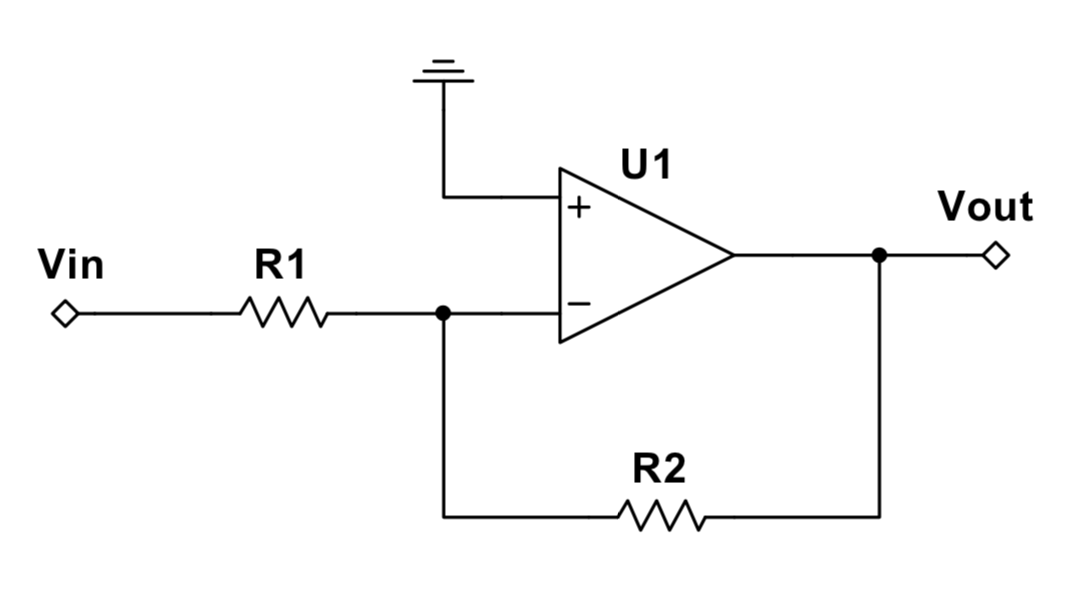
\includegraphics[width=2in]{opamps/inverting.png}
%	\caption{Inverting}
	\label{fig:fig}
\end{figure}
Gain equation:
\[\frac{V_{out}}{V_{in}} = -\frac{R_2}{R_1} \]

\section{Summer}
\begin{figure}[H]
	\centering
	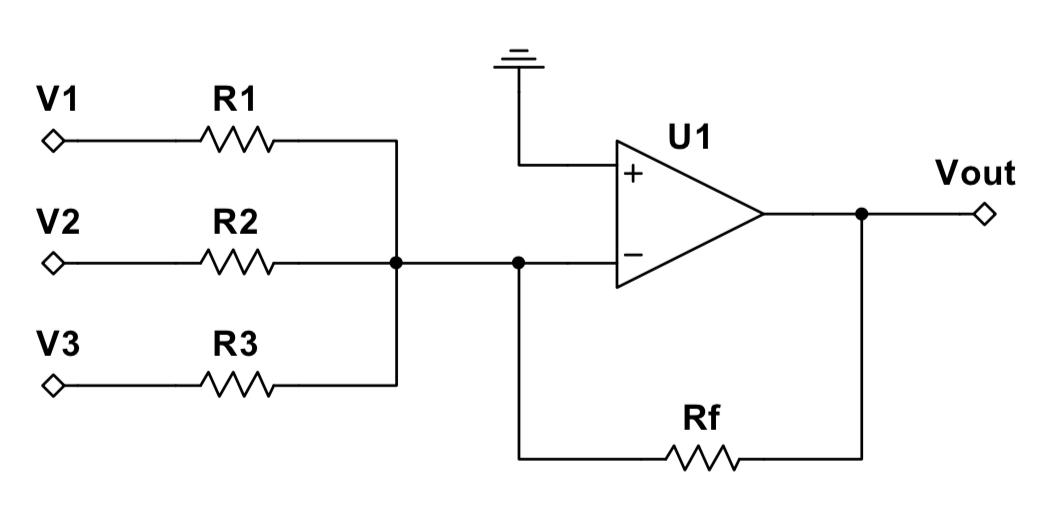
\includegraphics[width=2.5in]{opamps/summer.png}
%	\caption{Summer}
	\label{fig:fig}
\end{figure}
If $R_{in} =R_1=R_2=R_3$,
\[V_{out} = -\frac{R_f}{R_{in}}\left(V_1 + V_2 + V_3 + \cdots\right) \] 
Otherwise its a weighted summer, with equation
\[V_{out}= -\left(\frac{R_f}{R_1}V_1 + \frac{R_f}{R_2}V_2 + \cdots \frac{R_f}{R_n}V_n\right) \]


\section{Schmidt Trigger}
\begin{figure}[H]
	\centering
	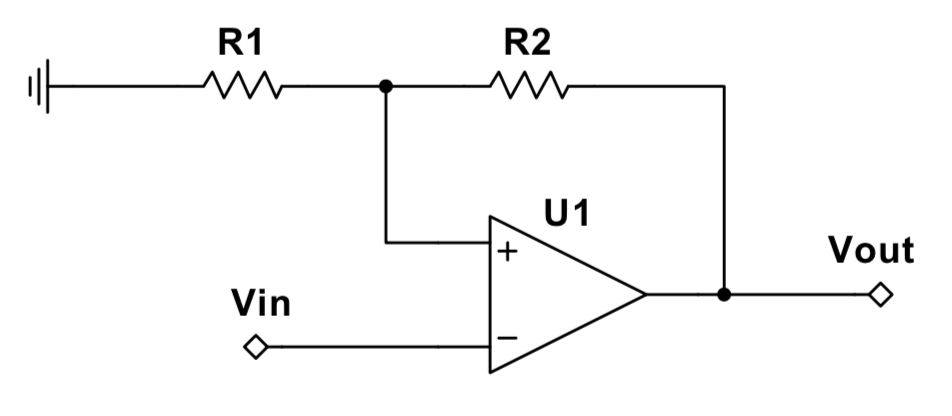
\includegraphics[width=2in]{opamps/schmidt.png}
%	\caption{Schmidt Trigger}
	\label{fig:fig}
\end{figure}
\todo{guardband}

\section{Oscillator}
\begin{figure}[H]
	\centering
	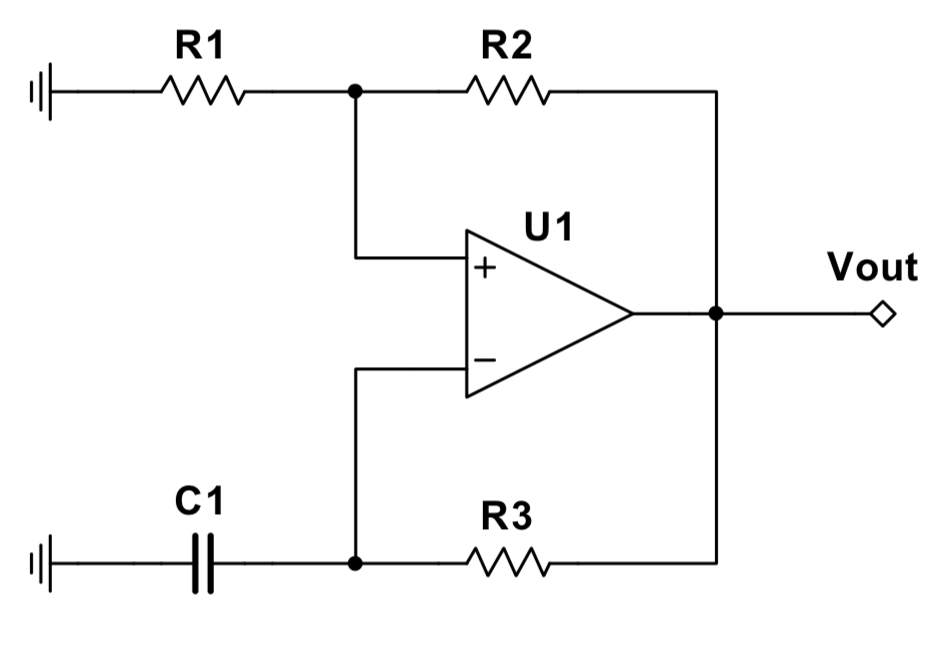
\includegraphics[width=2in]{opamps/oscillator.png}
%	\caption{Oscillator}
	\label{fig:fig}
\end{figure}
\todo{hysteresis}

\section{Integrator}
\begin{figure}[H]
	\centering
	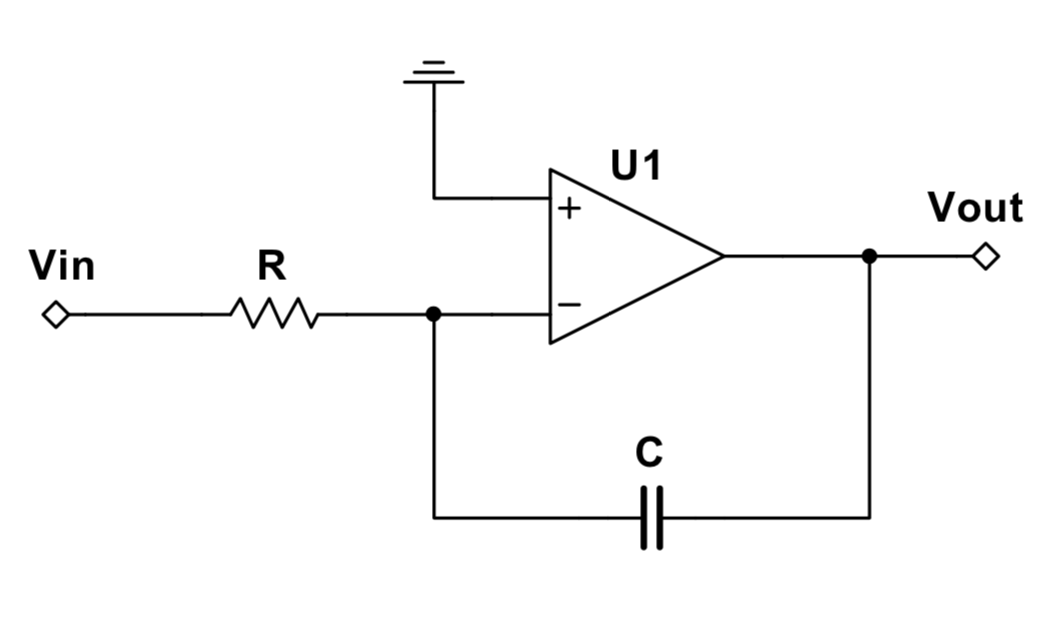
\includegraphics[width=2in]{opamps/integrator.png}
%	\caption{Integrator}
	\label{fig:fig}
\end{figure}
\[V_{out}= -\frac{1}{RC}\int_{0}^{t}V_{in}dt \]
\section{Differentiator}
\begin{figure}[H]
	\centering
	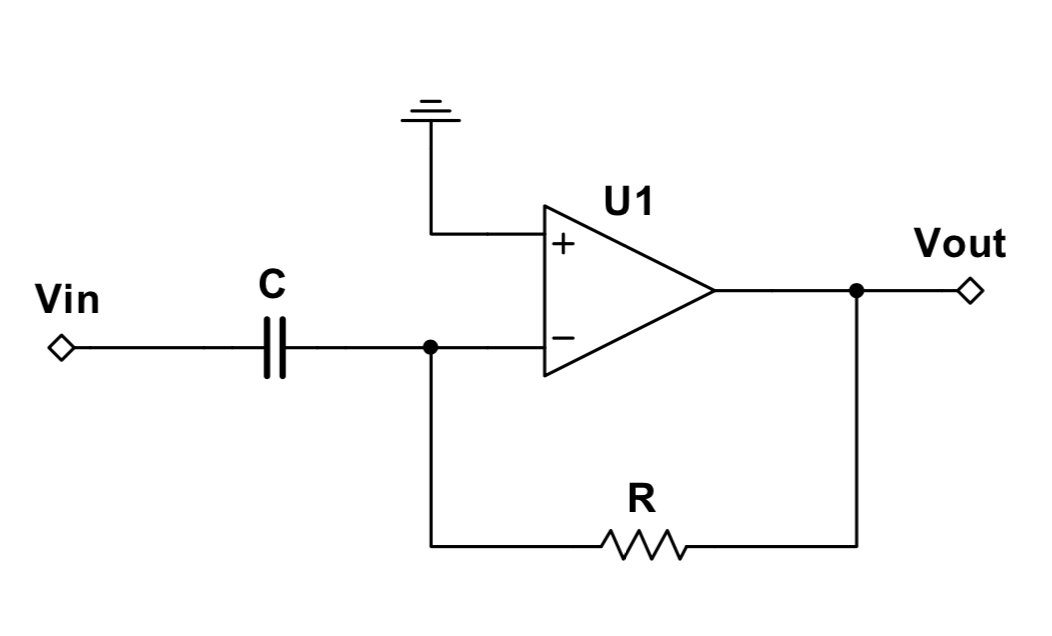
\includegraphics[width=2in]{opamps/differentiator.png}
%	\caption{Differentiator}
	\label{fig:fig}
\end{figure}
\[V_{out} = -RC\frac{dV_{in}}{dt} \]


\chapter{Diodes}

\section{Three Diode Models}
\begin{enumerate}
	\item Ideal model: no forward drop across the diode.
	\item \SI{0.7}{\V} model: In a resistor-diode circuit,
	\[I_D=\frac{V_S-V_D}{R}\]
	Where $V_D$ is a constant \SI{0.7}{\V}.
	\item Exponential model:
	\[I_D = I_{sat}\left(e^{V_D/V_{therm}}-1\right)\]
	In a resistor-diode circuit, set this equal to the KVL and solve for $V_D$:
	\begin{align*}
	I_D &= I_{sat}\left(e^{V_D/V_{therm}}-1\right)=\frac{V_S-V_D}{R} \\
	V_D &= V_T \ln\left(\frac{I}{I_{sat}}\right)
	\end{align*}
		
\end{enumerate}

\section{Log-Amp}
	\[V_{out}=-V_T \ln\left(\frac{V_{in}}{I_{sat}R}\right)\]

\chapter{MOSFETs}
\section{Recipie}
Recipie for solving transistor circuits
\begin{enumerate}
	\item Solve DC bias points ($V_{GS}$, $V_{DS}$, $I_{DQ}$)
	\item Calculate small signal parameters ($g_m$)
	\item Draw small signal model
	\item Solve for small signals
	\item Add DC + AC (small signals) to get full signal
\end{enumerate}
\textbf{Note:} We cannot calculate large signal values from small signal parameters \cite{ulaby}.

\section{Q-Point}
If $V_{GS} < V_{TN}$, the transistor is in Cutoff. Otherwise:
\begin{itemize}
	\item If $V_{DS} \leq V_{GS}-V_{TN}$, it's in Triode.
	\[I_{D}=k_n\left(V_{GS}-V_{TN}-\frac{V_{DS}}{2}\right)V_{DS}\]
	\item If $V_{DS} \geq V_{GS}-V_{TN}$, it's in Saturation.
	\[I_{D}=\frac{k_n}{2}\left(V_{GS}-V_{TN}\right)^2\]
\end{itemize}

\section{Transconductance}
\begin{equation}
g_m = k_n\left(V_{GS}-V_{TN}\right) = \sqrt{2k_n I_{D}} \label{eq:dis}
\end{equation}
Retrieved from \citeA{cad}.


\section{Small Signal Limit}
\[v_{gs}<0.2\left(V_{GS}-V_{TN}\right)\]
Usually have to do a KVL from here to get $v_{in}$.


\section{Common Source Small-Signal Gain}
	With source degeneration ($R_S$),
	\[A_v=\frac{-R_D||R_L \cdot g_m}{1+g_m R_S}\]
	Without,
	\[A_v=-R_D||R_L\cdot g_m\]

\section{Common Drain Small-Signal Gain}
	\[A_v=\frac{g_m\left(R_S||R_L\right)}{1+g_m\left(R_S||R_L\right)} \]

\chapter{BJTs}



\bibliographystyle{apacite}
\bibliography{ee}





\end{document}













